\subsection{Naive CUDA}

One simple way to implement CUDA parallel minimax is to launch CUDA threads to each potential move from the initial board state. Suppose we have a 15x15 board and lets assume that player 1 has played one move. Then, player 2 has $15\cdot 15-1=224$ potential moves from which to choose the optimal move. We can then launch 1 thread block of dimension \mintinline{C}{(224,1,1)} and have each thread of that block explore every potential move. \\
\\
As we will demonstrate in Section~\ref{sec:results}, this method severely underperforms in comparison to the CPU implementations for a couple of reasons, especially at higher search depths. The first is related to how our heuristic function is defined. Recall from Section~\ref{sec:minimax} that a static evaluation is calculated whenever the minimax algorithm encounters a terminal node or when the depth is equal to 0, signalling that we have gone as far as we want in the search tree. The heuristic function inevitably contains many if-else statements to account for different board configurations and states. Since in CUDA threads are run at the granularity of warps and since CUDA requires that each thread in a warp execute the same operation, this set of conditional operations causes thread divergence within the warp. This, of course, leads to sub-optimal performance from the GPU. \\
\\
Furthermore, and perhaps most importantly, 224 threads simply is not enough threads to see performance gains in CUDA. To extract good performance from the GPU, we need to use a thousands or tens of thousands of threads to hide latency and increase the chance of keeping the GPU busy. This second limitation of the naive GPU implementation motivates the sequential-parallel approach explained next.

\subsection{Sequential-parallel CUDA}
As mentioned the sequential-parallel CUDA implementation is an attempt to overcome the second limitation in the naive CUDA implementation. The main idea of this approach is to launch as many lightweight threads as possible. To this end, the sequential-parallel approach first splits the search tree of depth $d$ into two parts:
an upper part of depth $s$ and a lower part of depth $p$, where the upper part will be searched sequentially and the lower part will be searched in parallel. Note that $d=s+p$ must hold true. The lower part is then is divided into $k$ sub-trees and a GPU thread is launched for each of these $k$ sub-trees. Figure~\ref{fig:seqpar} provides graphic aid for the tree splitting.\\
\\
Now with this setup, the game tree search process takes 3 steps. \cite{Rocki}
\begin{enumerate}
    \item From the root node, sequentially search through depth $s$ and store the leaf board state into an array 
    \item For each of the leaves/board states, execute a parallel search of depth $p$.
    \item Traverse down the upper section of the tree retrieving the results from step 2 and finally return the best move.
\end{enumerate}

\begin{figure}[!htbp]
    \centering
    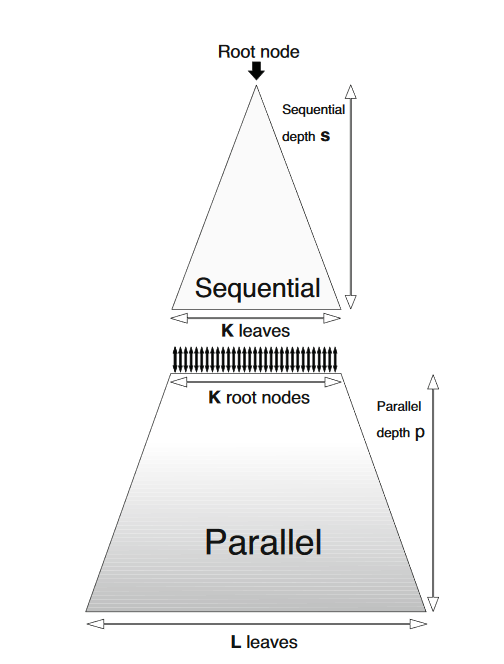
\includegraphics[scale=0.45]{images/seqpar.PNG}
    \caption{Parallelization strategy for sequential-parallel CUDA \cite{Rocki}}
    \label{fig:seqpar}
\end{figure}

\noindent
Since the original goal with the sequential-parallel method was to launch more lightweight threads, we can compare this method to the naive method with an example. Suppose again that we have a board of size 15x15 and player 1 has played one move. In the naive implementation, as explained in the previous section, we would launch 224 threads, each to explore some depth $d$. Note that the number of threads launched in the naive version is independent on $d$. Now suppose we set $d=3$ and we set $s=2, p=1$. This means we are exploring depth of 2 sequentially, and depth of 1 in parallel. In this scenario, we would instead launch $224\cdot 223=49952$ threads. As we can see, this is more in line with the general CUDA practice of launching more lightweight threads. In the sequential-parallel method, each GPU thread is responsible of depth of 1, whereas in the naive implementation each GPU thread would have been tasked with exploring a depth of 3 on its own. The difference in amount of work delegated to each thread, compounded with the effects of thread divergence as well, the sequential-parallel implementation leads to significant improvement compared to the naive implementation.\\
\\
One limitation/consideration that Rocki and Suda mention in their paper is that this strategy brings an overhead of having to execute the sequential tree section twice, once to populate the list of possible board states and once to retrieve the scores after the GPU threads calculate the scores.~\cite{Rocki} They further remark that due to this overhead, the choice of $s$ is important so that we can decrease the cost of this redundant operation, while generating enough leaves to saturate the GPU and its resources.




\subsection{PVS CUDA}
The problem with naive and the sequential-parallel CUDA implementation is that the result from earlier branches are used to determine whether later branches should be examined or not. If we search multiple branches in parallel, those branches do not have the bounds from each other to work with. This will result in searching unnecessary branches that will not lead to a solution. Therefore, we optimized our CUDA implementation by using PVS method from this paper \cite{pvsgpu}.\\

\noindent
Principle Variation Search (PVS) \cite{pvs} is a refinement of the alpha-beta pruning technique. The core idea is to assume the first examined move is the best and try to determine if a sub-tree will lead a cutoff. Before traversing through the tree further, a null-window search of the corresponding sub-tree is performed first. Null-window search means that the $\alpha$ and $\beta$ bounds are set to $\alpha = \alpha$ and $\beta = \alpha + 1$. Even if that means that the search will always fail, we will be able to determine if the earch will cause a $\beta$ cutoff or lies under $\alpha$ instead. If it fails, the sub-tree does not need to be searched any further, otherwise the sub-tree will be searched again with the result of the null-window search. The pseudo code of PVS is shown below.\\

\begin{algorithm}[!htbp]
\SetAlgoLined
\SetKwInOut{Input}{input}
\SetKwInOut{Output}{output}
\Input{nodes, $\alpha$, $\beta$, depth}
\Output{score}
\If{depth == 0}{
    return evaluate(n)\;
}
nodes = generate(n)\;
\If{nodes.isEmpty()}{
    return evalute(n)\;
}
score = PVS(nodes[0], $\beta$, $\alpha$, depth-1)\;
\For{j = 1 \KwTo nodes.size()-1}{
    \If{score $\geq$ $\beta$}{
        break\;
    }
    $\alpha$ = max(score, $\alpha$)\;
    value = PVS(nodes[j], $\alpha-1$, $\alpha$, depth-1)\;
    \If{value $>$ score}{
        \eIf{$\alpha$ $<$ value \& value $<$ $\beta$ \& depth $>$ 2}{
            score = PVS(nodes[j], $\beta$, value, depth-1)\;
        }{
            score = value\;
        }
    }
}
return score\;
\caption{PVS}
\label{alg:PVS}
\end{algorithm}

\noindent
This paper \cite{pvsgpu} has shown a hybrid approach of using both CPU and GPU. The leftmost branch is searched on the CPU, then the remaining child nodes will be searched on the GPU. This allows the GPU branches to use the bounds from CPU branch to avoid searching branches that would otherwise be pruned in serial implementation. Then we assign one block for each child node to search down the sub-tree rooted at the child node.\\

\begin{figure}[!htbp]
    \centering
    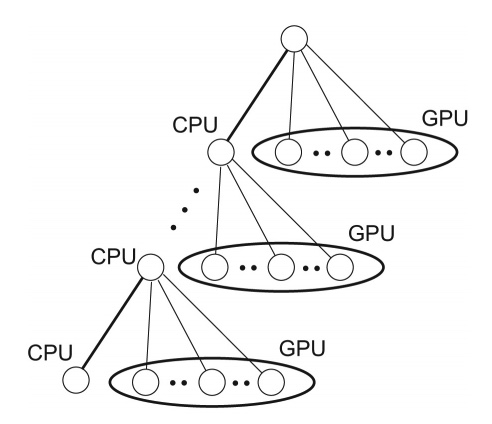
\includegraphics[scale=0.4]{images/pvs.jpg}
    \caption{CPU establishes bounds for GPU\cite{pvsgpu}}
\end{figure}

\begin{figure}[!htbp]
    \centering
    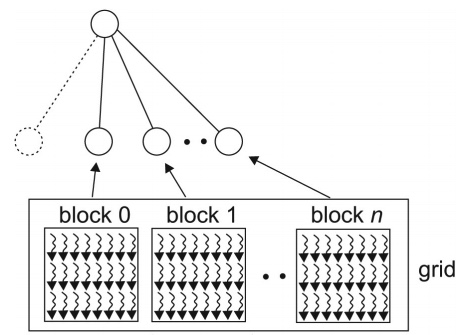
\includegraphics[scale=0.4]{images/pvs2.jpg}
    \caption{One block per child node\cite{pvsgpu}}
\end{figure}

\subsection{Dynamic Parallelism CUDA}
One problem with our PVS implementation is that we uses one block to fully search the entire sub-tree rooted at a child node. As depth increases, each block needs to search increasingly larger sub-trees. Therefore, we seek to fully parallelize our game tree search by using dynamic parallelism. \cite{dp}\\
\\
Dynamic Parallelism is a feature added in CUDA 5.0. It enables a CUDA kernel to create and synchronize new nested work, using the CUDA runtime API to launch other kernels, synchronize on kernel completion and perform device memory management, all without CPU involvement. \cite{dp2}\\
\\
In our implementation, our \textit{cudaSearchKernel} kernel function launches new kernels for each node to be searched. However, one possible trade off of this approach is the overhead of launching so many kernels.\\
